\section{Force control with various CKC formulations}\label{sec:2xminiJforce}

The purpose of this experiment is illustrating the differences of using the two different closed kinematic chain (CKC) formulations described in \ref{subsec:task-restrictions}. The first simulation is run with minimal CKCs, and the second one is run with the regular CKCs all defined with respect to the base frame.

The snake robot is in contact with three obstacles, whereas the force against the second and third obstacle is controlled. The desired force magnitude $f_{F,d}$ is 2 $N$ for both contacts. The simulation configuration is summarized in Table \ref{tab:exp_2xf} and is common for both simulations.

\begin{table}[]
    \centering
    \begin{tabular}{|c|c|c|}
        \hline
        & Value & Unit\\
        \hline
        Number of obstacles & $3$ & \\
        Number of links & $6$ & \\
        $f_{F,d}$ & $2$ & $N$ \\
        $[K_{p}, K_{i}]$ & $[0.5, 0.003]$ &\\
        \hline
    \end{tabular}
    \caption{Simulation configuration for force control experiment with minimal CKCs}
    \label{tab:exp_2xf}
\end{table}

It should be mentioned that very thorough tuning of control parameters could improve the results of both simulations, although a great deal of tuning already has been conducted. Furthermore, the control is quite twitchy as a result of the very varying force sensor feedback. The experiment in \ref{sec:pos-force-control-exp} is conducted with a low pass filtering of these sensor signals, and proves that the control consequently gets smoother as well.

\subsection{Regular CKCs}

For the first simulation, the regular CKC formulations are used. By regular it is here meant that all contact points are described with respect to the base frame of the robot. This setup is illustrated in Figure \ref{fig:CKC1} in \ref{subsec:task-restrictions}. It can be seen that the two CKCs for the second and third obstacle are overlapping. As a result, the first two joint motors will be utilized to reach the control goal for both contact points. The motors for joints 3 and 4 will however still be reserved the third contact point. From the input torque plot in Figure \ref{fig:2xf-bigJ} it can be seen that all joint motors except for the last one are actuated. The last one is left out as it is positioned after both the controlled contacts. 

Figure \ref{fig:2xf-bigJ} also shows the resulting contact forces. As expected, the contact forces for the third contact point are much better controlled than for the second contact point. This is because it has more actuators available, again making it more robust. In addition, it is known that the actuators used for the second contact point are shared for both controls. The input torques $\tau_3$ and $\tau_4$ used only for the third contact are clearly much more stable than the shared input torques $\tau_1$ and $\tau_2$.

Another reason for why $f_{F,2}$ never reaches its desired value can be that the joint torques related to this control reach the saturation limit, which has an absolute value of 2 in this experiment. Unfortunately, it was found that larger motor torques easily led to the contact being lost at some moments. This is highly undesired as the mathematical model assumes contact at all times.

\begin{figure}
    \centering
    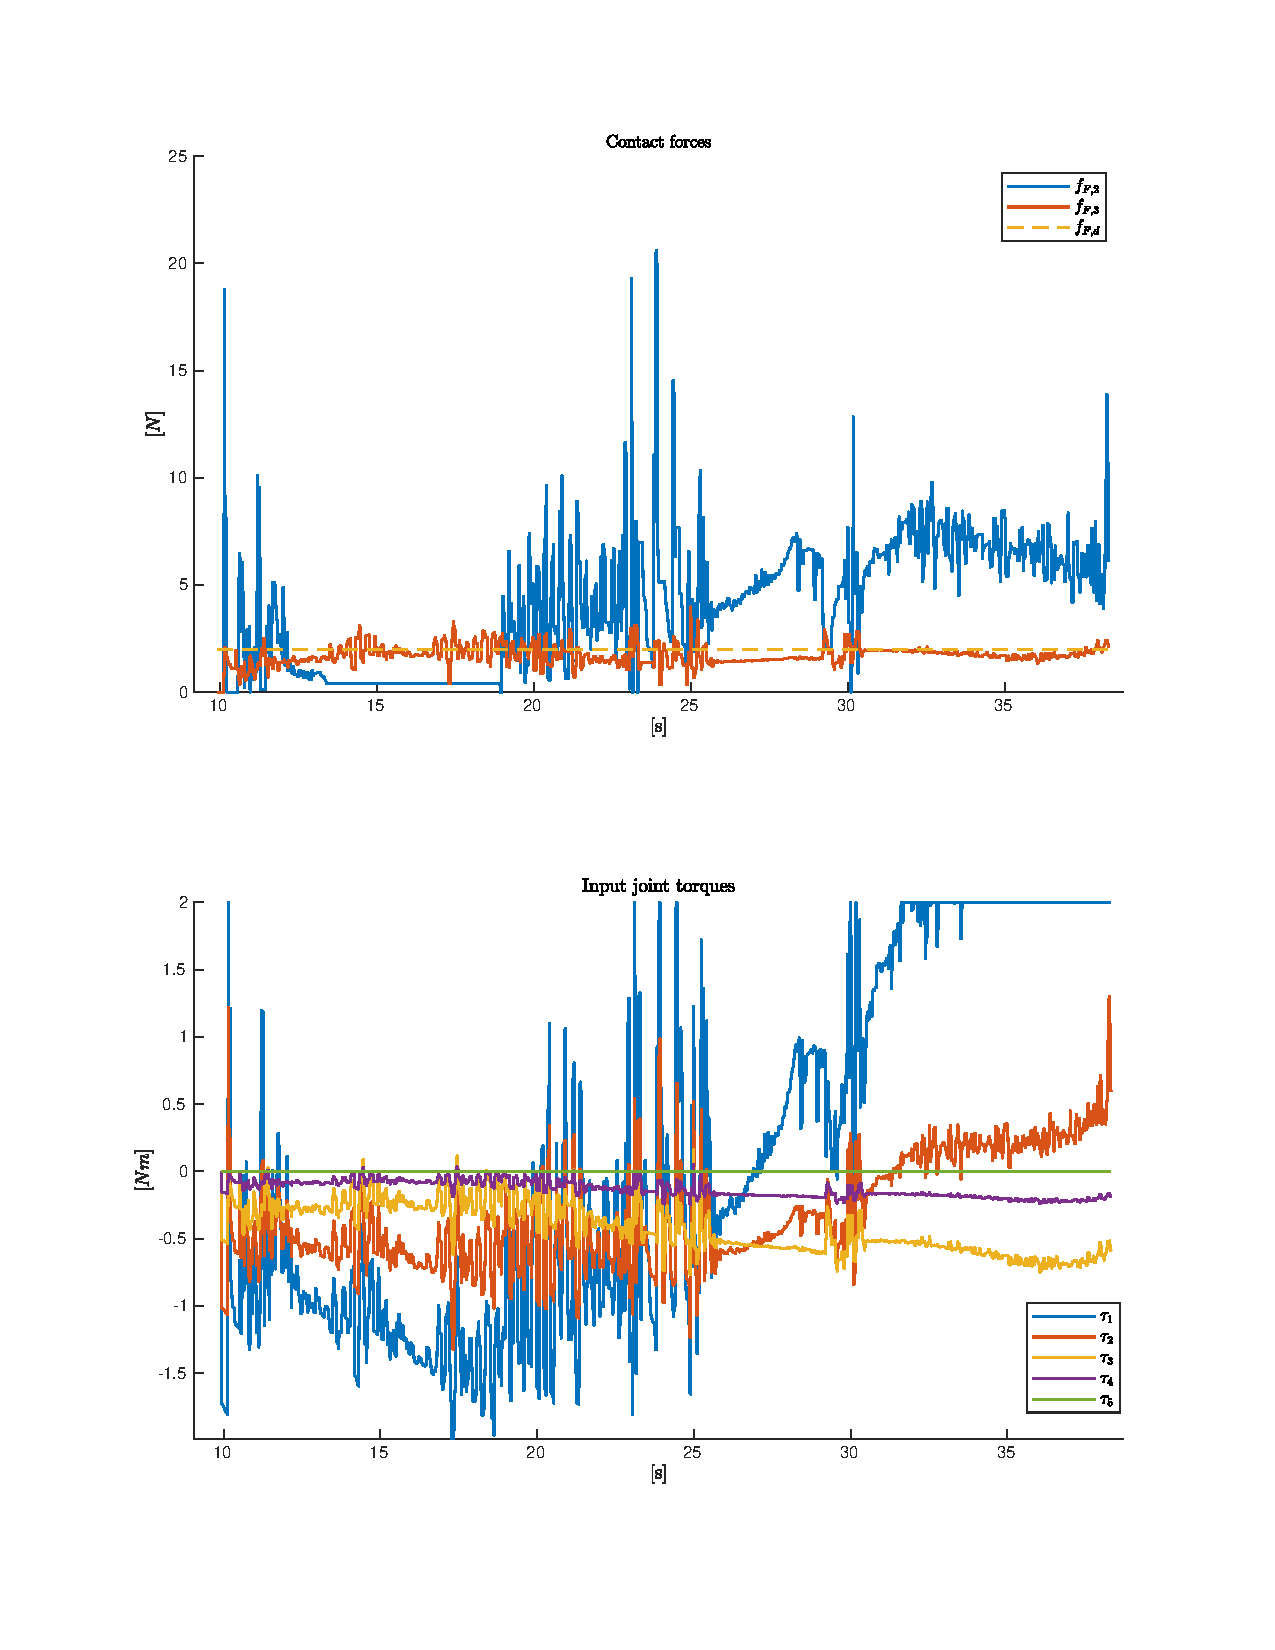
\includegraphics[trim=2cm 2cm 2cm 2cm, clip=true, width=\textwidth]{figures/experiments/2xf/bigJ-2plot.pdf}
    \caption{Experiment with regular CKCs}
    \label{fig:2xf-bigJ}
\end{figure}

\subsection{Minimal CKCs}

For the second simulation, the minimal CKC formulations are used. That means that the CKC for the second obstacle is defined from the first to the second obstacle point, and the CKC for the third obstacle is defined from the second to the third obstacle. This formulation is easier understood from the illustration in Figure \ref{fig:CKC2} in \ref{subsec:task-restrictions}. It can be observed that the CKC belonging to the third obstacle contains two joints, whereas the second one only has one joint.

Figure \ref{fig:2xf-miniJ} shows the resulting contact forces and joint torques from the simulation. From the figure it can be seen that both forces are close to the desired value. Nonetheless, the force against the third obstacle ($f_{F,3}$) is considerably more stable than the one against the second obstacle ($f_{F,2}$). It is not implausible that this is a result of the third contact point having one more joint available for control. This increases the robustness of the control. In addition, it is known that the joint connecting link 3 and 4 will influence the third link. This can further be seen as a disturbance on the control of the second contact force.

\begin{figure}
    \centering
    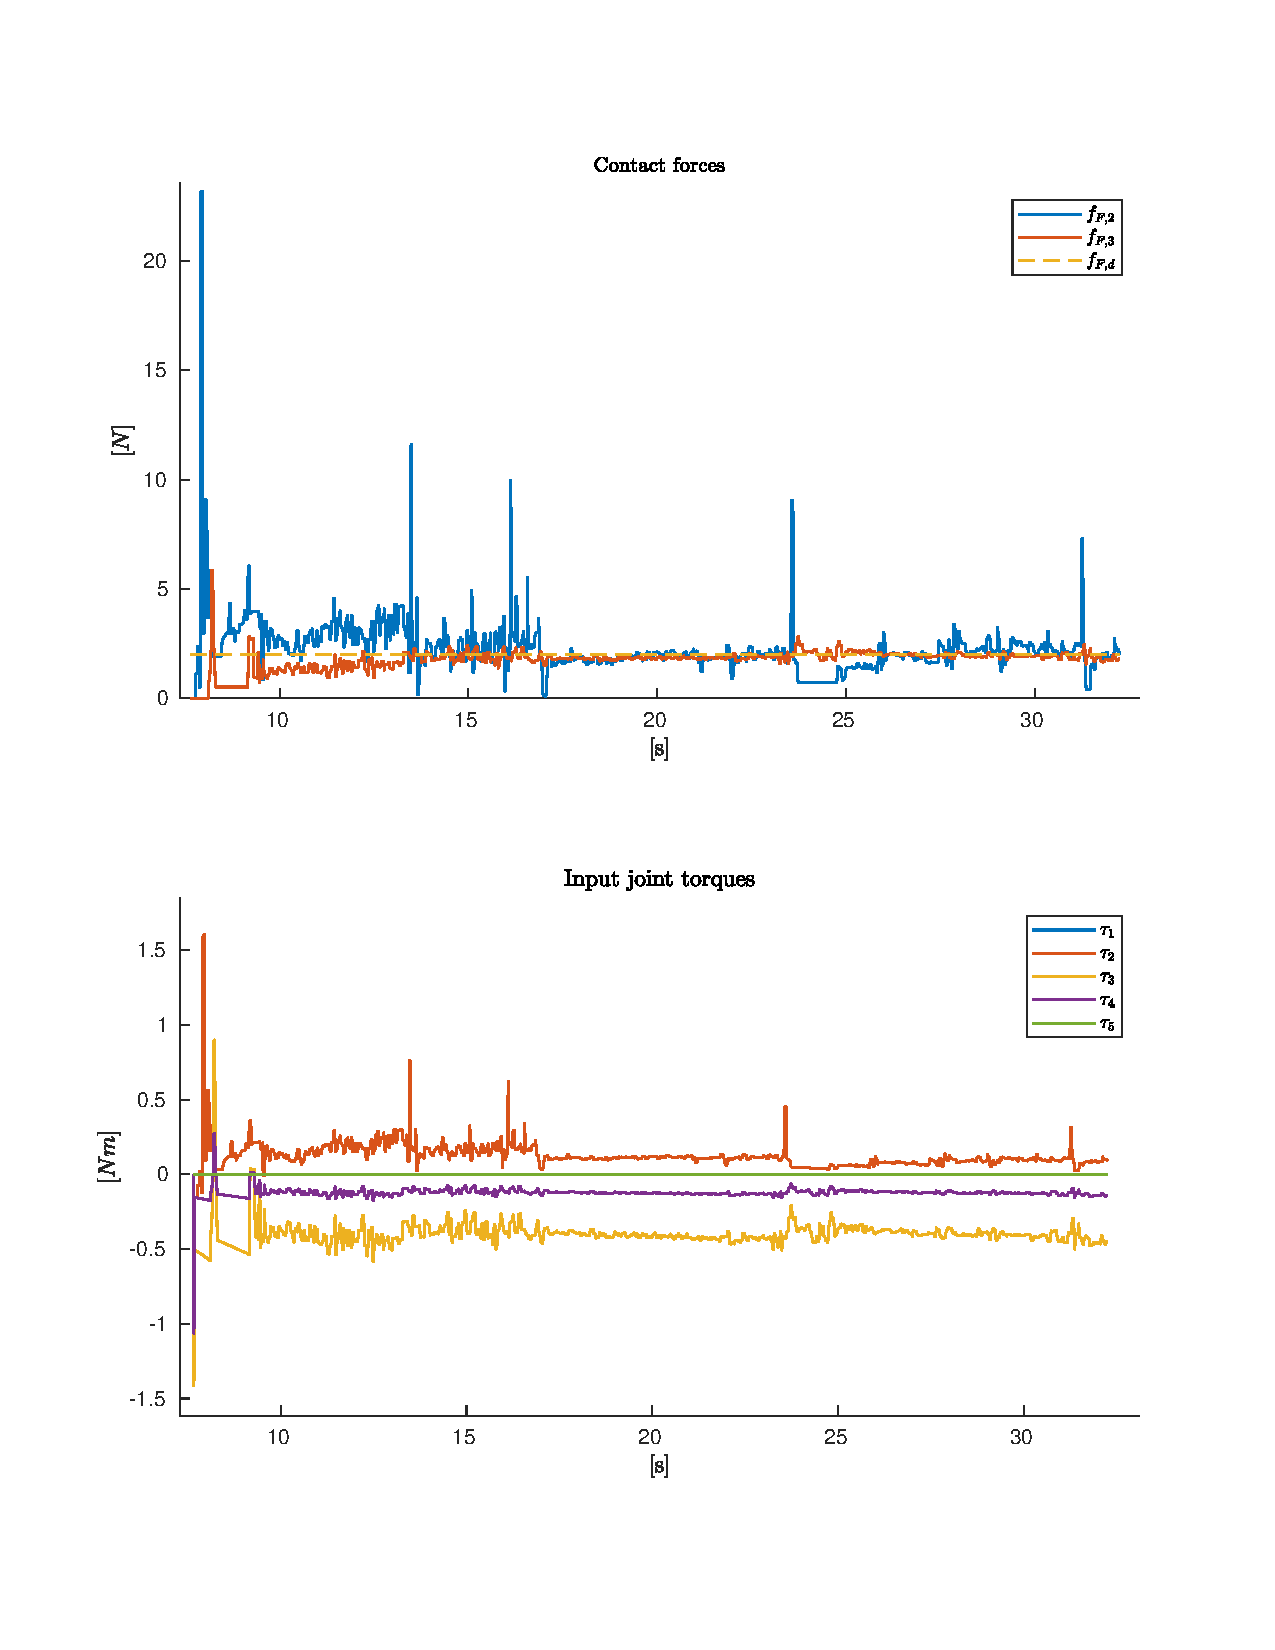
\includegraphics[trim=2cm 2cm 2cm 2cm, clip=true, width=\textwidth]{figures/experiments/2xf/miniJ-2plot.pdf}
    \caption{Experiment with minimal CKCs}
    \label{fig:2xf-miniJ}
\end{figure}

From the control torques in Figure \ref{fig:2xf-miniJ}, it is evident that only the motors on joints 2, 3 and 4 are used. This is logical, as it is exactly what the corresponding CKCs allow. Since the controllability increases with the current CKC definition, the control is also significantly smoother than in the previous simulation.



%Filtering the sensor signals with a low pass filter could have improved the smoothness of the results. However, the main sense of the experiment is still communicated with the presented results.

